\chapter{CloudyRSS}
Simulations and small tests conducted in a controlled environment are a
good way to evaluate the effectiveness of complex infrastructures as the
one displayed by \cloudcast. However only data gathered via a
deployed system can provide a realistic picture.
Keeping this in mind the final work performed during this thesis
has been directed to develop a simple yet realistic application based
on the \cloudypeer framework and exploiting the \cloudcast
architecture.

News distribution, in the form of \textit{RSS} feeds, has been chosen as
the target scenario since it perfectly fits the proposed
approach: it features a central component with a dynamic set of
updates to be distributed to a potentially huge collection of nodes.
The literature shows multiple works where \ptop techniques
have been applied to the \textit{RSS} distribution
problem~\cite{P2PFeedDelivery}
\cite{AttackResilientP2PFeedDissemination}
\cite{SimpleSecurityP2PFeedDissemination}, however to the best of our
knowledge none tries to conciliate the central nature of the problem
with the \ptop component.

The result of this effort is an application called \cloudyrss which
allow standard \textit{RSS reader} software to fetch their news via a
\cloudcast based system.

\begin{figure}[h!]
  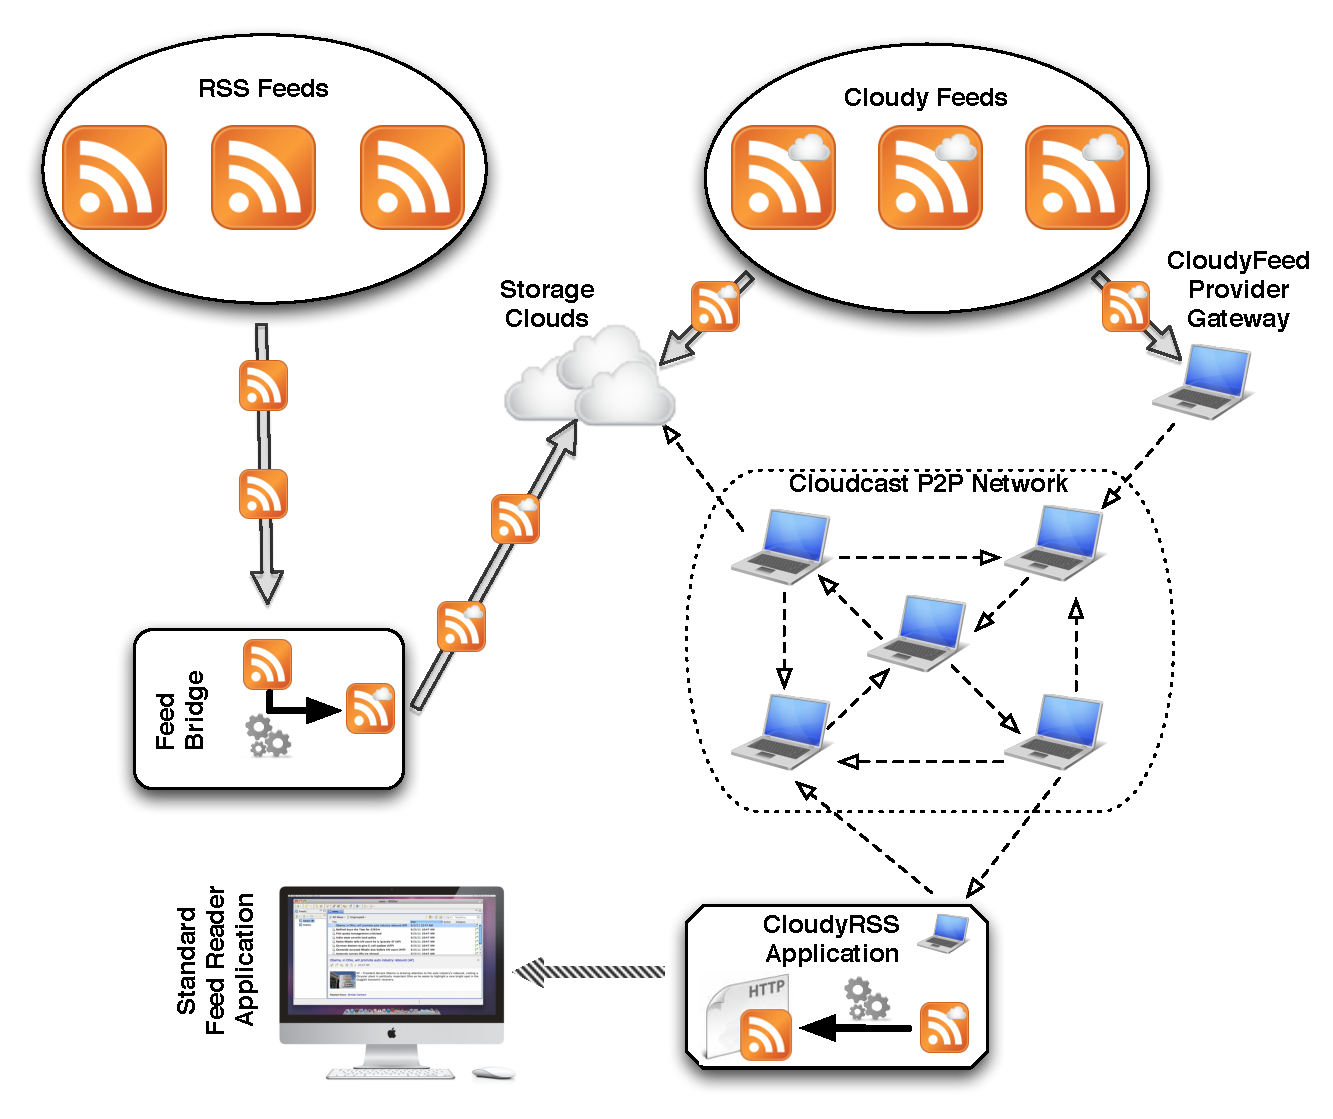
\includegraphics[width=\textwidth]{cloudyrss-architecture.pdf}
  \caption{Architectural overview of \cloudyrss}
  \label{fig:cloudyrss-architecture}
\end{figure}

Figure~\ref{fig:cloudyrss-architecture} shows a general overview of
the system. As can be noted the news sources are divided in two
categories. The first is represented by the \cloudyrss-aware sources
which are fully integrated in the system: their updates are distributed
by placing them on the \cloud and/or by employing a gateway node
responsible of starting the \epidemic diffusion.
The second category embodies all the standard \textit{RSS} feed
sources: these are not directly involved in the architecture; instead their
updates are collected by an entity called \textit{Feed
  Bridge} which converts them in \cloudyrss compatible news and place
them on the \cloud.

Once the updates are entered in the system, \cloudcast takes care of
delivering them to all subscribed nodes where they are converted back in
\textit{RSS} form and offered via a local web server instance to the
\textit{RSS reader} software of choice.

\begin{figure}[h!]
  \centering
  \subfloat[][\cloudyrss\ status window showing ``news'' feed URL]{
    \hspace{-70pt}
    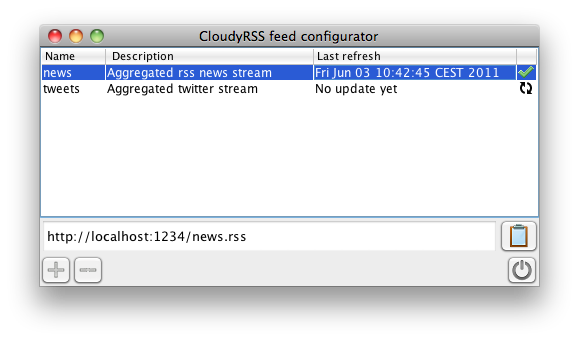
\includegraphics[width=240pt]{cloudyrss-main.png}
    \label{fig:cloudyrss-main}
  }
  \subfloat[][RssOwl properties window for feed ``news'']{
    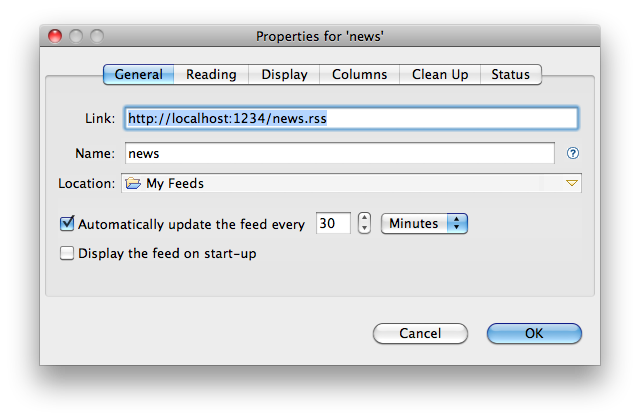
\includegraphics[width=240pt]{cloudyrss-properties.png}
    \label{fig:cloudyrss-properties}
  }
  \caption{Feeds' URLS configuration in an RSS reader}
  \label{fig:cloudyrss-feeds}
\end{figure}

\clearpage
Users can subscribe to a news feed by loading a
configuration file equivalent to the ``.torrent'' one used by
\textit{BitTorrent} softwares. Once the desired feed have been
added, the \textit{RSS reader} must be configured to use them.
Figures~\ref{fig:cloudyrss-main} and~\ref{fig:cloudyrss-properties}
shows this process: the URL of the \textit{RSS file} generated by
\cloudypeer is copied from the main application window and entered in
the feed configuration window of the \textit{RSS reader}.
The end result is that the news obtained via the \cloudcast system are
transparently displayed in the \textit{RSS reader} as shown in
figure~\ref{fig:cloudyrss-view}

Thanks to this system is possible to setup experiments confronting the
costs of distributing the \textit{RSS} file with the
\cloudcast based system with respect to the standard strategy. The actual
planning and realization of such tests is however out of the scope of
this work and thus will not be analyzed further.

Once again the code of \cloudyrss is available via a \github
repository~\cite{cloudyrss-repo} with the last version at the time of
this writing tagged with \thesistag.

\begin{figure}[h!]
  \hspace{-40pt}
  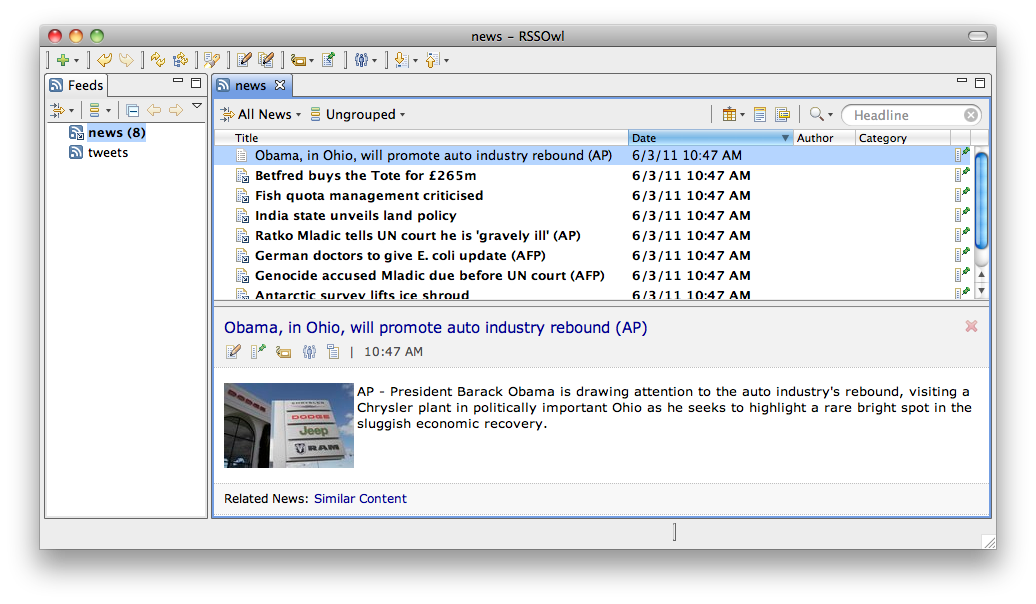
\includegraphics[width=1.2\textwidth]{cloudyrss-view.png}
  \caption{RssOwl main windows showing the ``news'' feed obtained
    through \cloudyrss}
  \label{fig:cloudyrss-view}
\end{figure}
